\documentclass{beamer}
\usepackage{../common_slides}
\usepackage{tikz}
\usepackage{tikz-qtree}
\usepackage{pdfpages}

\usetikzlibrary{bayesnet,matrix}
% \usepackage{enumitem}

\title{Sequence Models 2}
\date{}
\author{CS 287}

\def\Lattice{
    \matrix (network)
    [matrix of nodes,
    nodes in empty cells,
    ampersand replacement=\&,
    column sep={1cm},
    row sep={0.1cm},
    nodes={outer sep=0pt,circle,minimum size=0.5cm, minimum width=1.3cm,draw, rectangle} ]
    {
     O \& O \& O \& O \& O\\
     I-PER \& I-PER \& I-PER \& I-PER \& I-PER \\ 
     I-ORG \& I-ORG \& I-ORG \& I-ORG \& I-ORG \\ 
     I-LOC \& I-LOC \& I-LOC \& I-LOC \& I-LOC \\ 
     |[draw=none]| \\
     |[draw=none]| Mayor \& |[draw=none]| DeBlasio \& |[draw=none]| from \& |[draw=none]| New  \& |[draw=none]| York  \\  
};
}

\begin{document}

\begin{frame}
  \titlepage
\end{frame}



\begin{frame}{Review: Hidden Markov Model}
\begin{center}  
  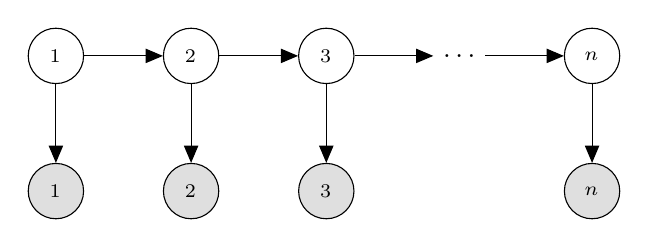
\begin{tikzpicture}
    \node (Ea) [obs] {$\boldx_1$}; 
    \node (Xa) [latent,above =of Ea] {$\boldy_1$}; 

    \node (Eb) [obs, right = of Ea ] {$\boldx_2$}; 
    \node (Xb) [latent,above =of Eb] {$\boldy_2$}; 

    \node (Ec) [obs, right = of Eb] {$\boldx_3$}; 
    \node (Xc) [latent,above =of Ec] {$\boldy_3$}; 
    \node (Xd) [right =of Xc] {$\ldots$}; 
    \node (Xe) [latent,right =of Xd] {$\boldy_n$}; 
    \node (Ee) [obs,below =of Xe] {$\boldx_n$}; 

    \edge {Xa} {Xb} ; %
    \edge {Xb} {Xc} ; %
    \edge {Xa} {Ea} ; %
    \edge {Xb} {Eb} ; %
    \edge {Xc} {Ec} ; %
    \edge {Xc} {Xd} ; %
    \edge {Xd} {Xe} ; %
    \edge {Xe} {Ee} ; %
  \end{tikzpicture}
\end{center}  
\end{frame}


\begin{frame}{Review: Hidden Markov Model}
  Hidden Markov model requires two distributions,
  \begin{itemize}
  \item Transition distribution 
    \[p(\boldy_i | \boldy_{i-1}; \theta)\]
  \item Emission distribution
    \[ p(\boldx_i | \boldy_i ; \theta)\] 
  \end{itemize}


  \begin{itemize}
  \item How many total parameters?
  \end{itemize}
\end{frame}


\begin{frame}{Review: Maximum Entropy Markov Model}
  MEMM estimates only a transition distribution,
  \begin{itemize}
  \item Transition distribution (also conditioned on input)
    \[p(\boldy_i | \boldy_{i-1}=\delta(c_{i-1}), \boldx_1, \ldots, \boldx_n) = \softmax(feat(\boldx, c_{i-1}) \boldW + \boldb) \]

  \item Here $feat$ is a deterministic combination of the input and the previous $c_{i-1}$   
  \end{itemize}
  \begin{itemize}
  \item How many total parameters?
  \end{itemize}
\end{frame}


\begin{frame}{History-Based Model}
  \begin{itemize}
  \item In general, intractable to solve sequence prediction,
 
  \[ \argmax_{c_{1:n}} f(\boldx, c_{1:n}) \] 

  \item Today, focus on (first-order) history-based models,

  \[ f(\boldx, c_{1:n})  = \sum_{i=1}^n \hat{\boldy}(c_{i-1})_{c_i}\] 

  \item Can extend these ideas to higher-order models.

  \[ f(\boldx, c_{1:n})  = \sum_{i=1}^n \hat{\boldy}(c_{i-2}, c_{i-1})_{c_i}\] 
  \end{itemize}  
  
\end{frame}

\begin{frame}{Quiz: History-Based Models}
  Given this definition of a history-based model, 

  \[ f(\boldx, c_{1:n})  = \sum_{i=1}^n \log \hat{\boldy}(c_{i-1})_{c_i} \] 

  Describe the function $g$ for the following models, 

  \begin{enumerate}
  \item Hidden Markov Model
  \item Maximum-Entropy Markov Model
  \item Bigram Language Model (with no $\boldx$, e.g. best $n$ babble)
  \item NNLM with $\dwin=1$
  \end{enumerate}
\end{frame}


\begin{frame}{Answers}
  \begin{itemize}
  \item HMM
    \begin{eqnarray*}
      \log \hat{\boldy}(c_{i-1})_{c_i} &=& \log p(\boldy_i = \delta(c_{i}) | \boldy_{i-1}=\delta(c_{i-1})) + \log p(\boldx_i| \boldy_i )  \\
                                       &=& \log T_{c_{i-1}, c_i}  + \log E_{x_i, c_i}
    \end{eqnarray*}


    \pause 

  \item MEMM
    \[\log \hat{\boldy}(c_{i-1}) = \log \softmax(feat(\boldx, c_{i-1}) \boldW + \boldb)  \]
    \pause 

  \item Bigram 
    \[\log \hat{\boldy}(c_{i-1})_{c_i} = \log p(\boldy_i = \delta(c_{i}) | \boldy_{i-1}=\delta(c_{i-1}))  \]
    \pause 

  \item NNLM 
    \[\log \hat{\boldy}(c_{i-1}) = \log \softmax(\tanh(v(c_{i-1}) \boldW^1 + \boldb^1) \boldW^2 + \boldb^2)  \]

  \end{itemize}
\end{frame}

\section{}

\begin{frame}
  \begin{center}
   
  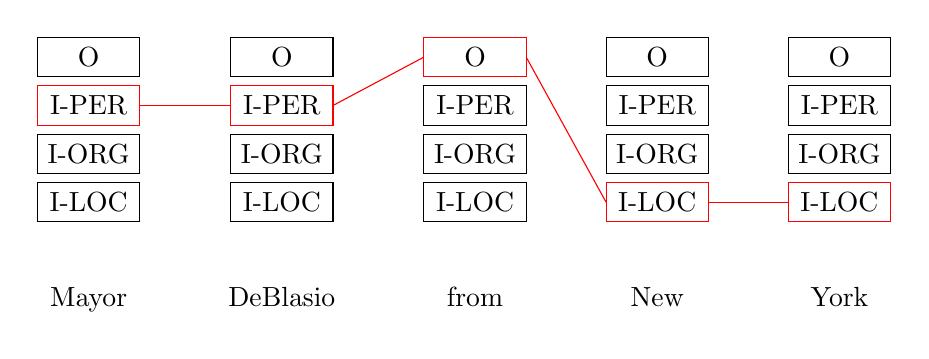
\begin{tikzpicture}
    \Lattice
    \draw[red] (network-2-1.north west) rectangle  (network-2-1.south east);
    \draw[red] (network-2-2.north west) rectangle  (network-2-2.south east);
    \draw[red] (network-1-3.north west) rectangle  (network-1-3.south east);
    \draw[red] (network-4-4.north west) rectangle  (network-4-4.south east);
    \draw[red] (network-4-5.north west) rectangle  (network-4-5.south east);

    \draw[red] (network-2-1.east) --  (network-2-2.west);
    \draw[red] (network-2-2.east) -- (network-1-3.west); 
    \draw[red] (network-1-3.east) -- (network-4-4.west);
    \draw[red] (network-4-4.east) -- (network-4-5.west);
    
  \end{tikzpicture}
  \end{center}
      % |[draw=none]| & |[xshift=1mm]| & |[xshift=-1mm]| \\
\end{frame}


\begin{frame}
  \begin{center}
   
  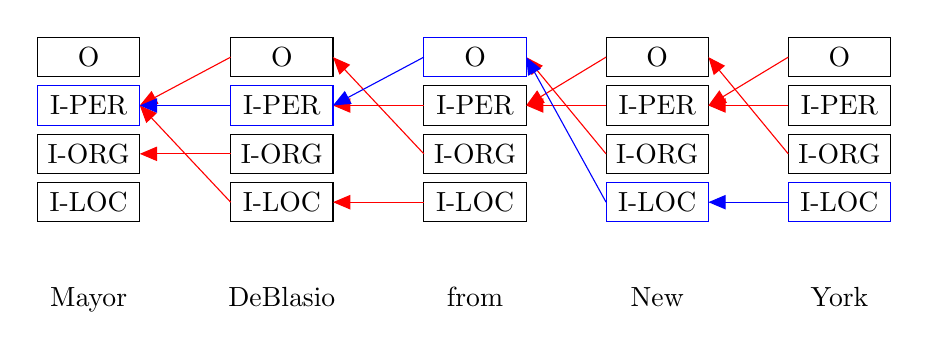
\begin{tikzpicture}
    \Lattice

    \draw[red,<-] (network-2-1.east) --  (network-1-2.west);

    \draw[red,<-] (network-3-1.east) --  (network-3-2.west);
    \draw[red,<-] (network-2-1.east) --  (network-4-2.west);
    \draw[blue,<-] (network-2-1.east) --  (network-2-2.west);


    \draw[red,<-] (network-2-2.east) --  (network-2-3.west);
    \draw[red,<-] (network-1-2.east) --  (network-3-3.west);
    \draw[red,<-] (network-4-2.east) --  (network-4-3.west);
    \draw[blue,<-] (network-2-2.east) --  (network-1-3.west);

    \draw[red,<-] (network-2-3.east) --  (network-1-4.west);
    \draw[red,<-] (network-2-3.east) --  (network-2-4.west);
    \draw[red,<-] (network-1-3.east) --  (network-3-4.west);
    \draw[blue,<-] (network-1-3.east) --  (network-4-4.west);

    \draw[red,<-] (network-2-4.east) --  (network-1-5.west);
    \draw[red,<-] (network-2-4.east) --  (network-2-5.west);
    \draw[red,<-] (network-1-4.east) --  (network-3-5.west);
    \draw[blue,<-] (network-4-4.east) --  (network-4-5.west);

    \draw[blue] (network-2-1.north west) rectangle  (network-2-1.south east);
    \draw[blue] (network-2-2.north west) rectangle  (network-2-2.south east);
    \draw[blue] (network-1-3.north west) rectangle  (network-1-3.south east);
    \draw[blue] (network-4-4.north west) rectangle  (network-4-4.south east);
    \draw[blue] (network-4-5.north west) rectangle  (network-4-5.south east);


    % \draw[red] (network-2-1.east) --  (network-1-2.west);
    % \draw[red] (network-2-1.east) --  (network-2-2.west);
    % \draw[red] (network-3-1.east) --  (network-3-2.west);
    % \draw[red] (network-2-1.east) --  (network-4-2.west);


    
  \end{tikzpicture}
  \end{center}
      % |[draw=none]| & |[xshift=1mm]| & |[xshift=-1mm]| \\
\end{frame}



\begin{frame}
  \begin{center}
   
  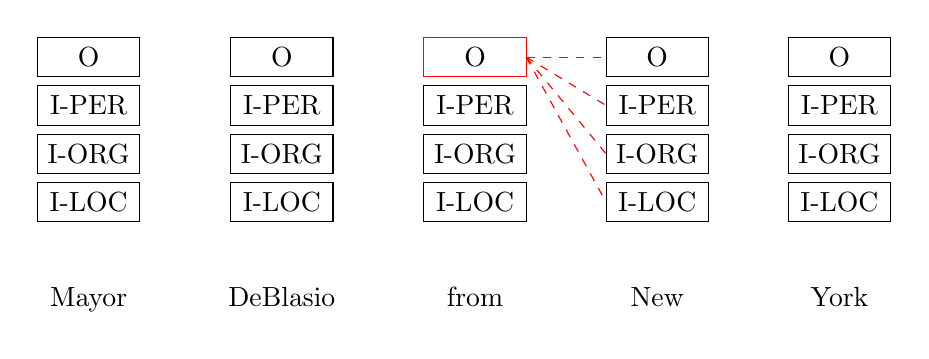
\begin{tikzpicture}
    \Lattice
    \draw[red] (network-1-3.north west) rectangle  (network-1-3.south east);

    \draw[red,dashed] (network-1-3.east) -- (network-1-4.west);
    \draw[red,dashed] (network-1-3.east) -- (network-2-4.west); 
    \draw[red,dashed] (network-1-3.east) -- (network-3-4.west);
    \draw[red,dashed] (network-1-3.east) -- (network-4-4.west);
  \end{tikzpicture}
  \end{center}
      % |[draw=none]| & |[xshift=1mm]| & |[xshift=-1mm]| \\
\end{frame}


\begin{frame}
  \begin{center}
   
  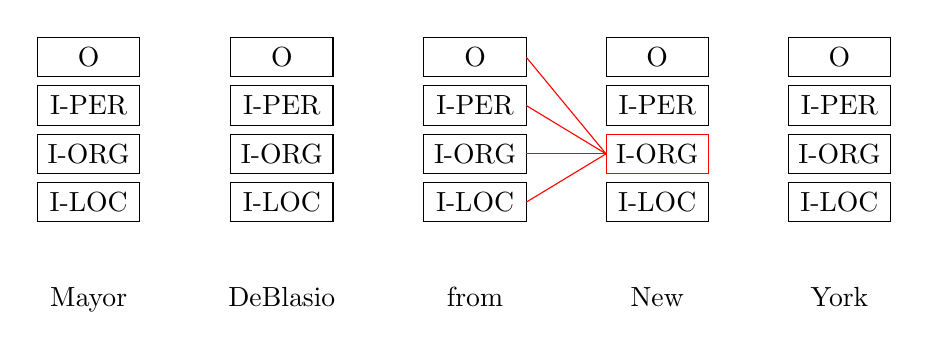
\begin{tikzpicture}
    \Lattice
    \draw[red] (network-3-4.north west) rectangle  (network-3-4.south east);

    \draw[red] (network-1-3.east) -- (network-3-4.west);
    \draw[red] (network-2-3.east) -- (network-3-4.west); 
    \draw[red] (network-3-3.east) -- (network-3-4.west);
    \draw[red] (network-4-3.east) -- (network-3-4.west);
  \end{tikzpicture}
  \end{center}
      % |[draw=none]| & |[xshift=1mm]| & |[xshift=-1mm]| \\
\end{frame}



\begin{frame}
  \begin{center}
   
  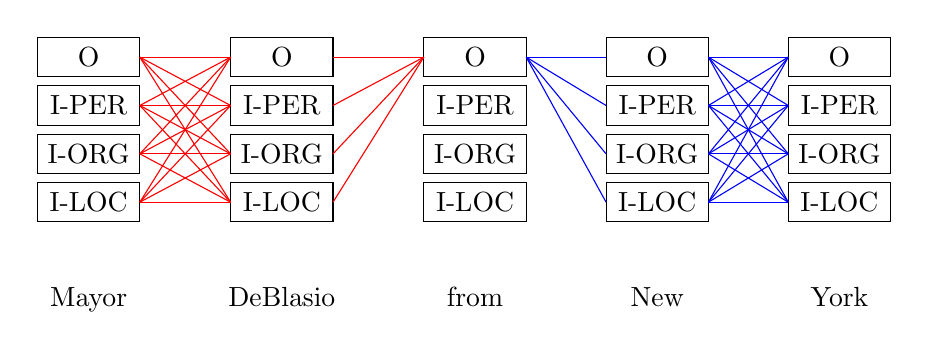
\begin{tikzpicture}
    \Lattice

    \draw[blue] (network-1-3.east) -- (network-1-4.west);
    \draw[blue] (network-1-3.east) -- (network-2-4.west); 
    \draw[blue] (network-1-3.east) -- (network-3-4.west);
    \draw[blue] (network-1-3.east) -- (network-4-4.west);

    \draw[red] (network-1-3.west) -- (network-1-2.east);
    \draw[red] (network-1-3.west) -- (network-2-2.east); 
    \draw[red] (network-1-3.west) -- (network-3-2.east);
    \draw[red] (network-1-3.west) -- (network-4-2.east);

    \foreach \i in {1,...,4} {
    \foreach \j in {1,...,4} {
    \draw[red] (network-\i-1.east) -- (network-\j-2.west);
    % \draw[red] (network-\i-2.east) -- (network-\j-3.west);
    % \draw[red] (network-\i-3.east) -- (network-\j-4.west);
    \draw[blue] (network-\i-4.east) -- (network-\j-5.west);
    } }

  \end{tikzpicture}
  \end{center}  
\end{frame}


\begin{frame}{Edge Marginal}
  \begin{center}
   
  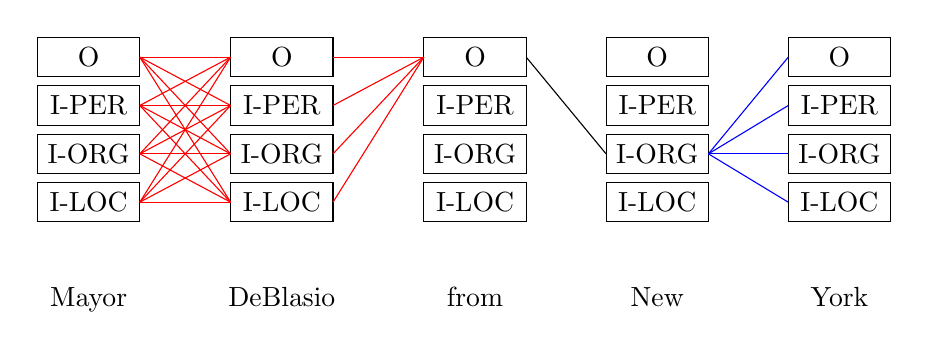
\begin{tikzpicture}
    \Lattice

    \draw[blue] (network-3-4.east) -- (network-1-5.west);
    \draw[blue] (network-3-4.east) -- (network-2-5.west); 
    \draw[blue] (network-3-4.east) -- (network-3-5.west);
    \draw[blue] (network-3-4.east) -- (network-4-5.west);
    \draw[black] (network-1-3.east) -- (network-3-4.west);

    \draw[red] (network-1-3.west) -- (network-1-2.east);
    \draw[red] (network-1-3.west) -- (network-2-2.east); 
    \draw[red] (network-1-3.west) -- (network-3-2.east);
    \draw[red] (network-1-3.west) -- (network-4-2.east);

    \foreach \i in {1,...,4} {
    \foreach \j in {1,...,4} {
    \draw[red] (network-\i-1.east) -- (network-\j-2.west);
    % \draw[red] (network-\i-2.east) -- (network-\j-3.west);
    % \draw[red] (network-\i-3.east) -- (network-\j-4.west);
    % \draw[blue] (network-\i-4.east) -- (network-\j-5.west);
    } }

  \end{tikzpicture}
  \end{center}  
\end{frame}


\begin{frame}
  
\end{frame}



\begin{frame}{Viterbi Algorithm (Simple)}
  \begin{algorithmic}
    \Procedure{Viterbi}{}
    \State{$\pi \in \reals^{\{0,\ldots, n\} \times \mcC}$ initialized to $-\infty$ }
    \State{$\pi[0, \langle s \rangle] = 0$}
    \For{$i = 1$ to $n$ }
    \For{$c_{i} \in \mcC$}
    \State{$\pi[i, c_i] = \max_{c_{i-1}} 
     \pi[i-1, c_{i-1}] + \log \hat{\boldy}(c_{i-1})_{c_i}        
       $}
    \EndFor{}
    \EndFor{}
    \State{\Return{$\max_{c_n\in\mcC} \pi[n, c_n]$}}
    \EndProcedure{}
  \end{algorithmic}
\end{frame}

\begin{frame}{Viterbi Algorithm with Precompute}
  \begin{algorithmic}
    \Procedure{ViterbiWithPrecompute}{}
    \State{$\pi \in \reals^{\{0,\ldots, n\} \times \mcC}$ initialized to $-\infty$ }
    \State{$\pi[0, \langle s \rangle] = 0$}
    \For{$i = 1$ to $n$ }
    \For{$c_{i-1} \in \mcC$}
    \State{precompute \alert{$\hat{\boldy}(c_{i-1})$}}
    \For{$c_{i} \in \mcC$}
    \State{$score = \pi[i-1, c_{i-1}] + \log \hat{\boldy}(c_{i-1})_{c_i} $}
    \If{$score > \pi[i, c_i]$}
    \State{$\pi[i, c_i] = score$}
    \EndIf{}
    \EndFor{}
    \EndFor{}
    \EndFor{}
    \State{\Return{$\max_{c_n\in\mcC} \pi[n, c_n]$}}
    \EndProcedure{}
  \end{algorithmic}

\end{frame}




\begin{frame}{Viterbi Algorithm with Backpointers}
  \begin{algorithmic}
    \Procedure{ViterbiWithBP}{}
    \State{$\pi \in \reals^{\{0,\ldots, n\} \times \mcC}$ initialized to $-\infty$ }
    \State{\alert{$bp \in \mcC^{\{1,\ldots, n\} \times \mcC}$} initialized to $\epsilon$ }
    \State{$\pi[0, \langle s \rangle] = 0$}
    \For{$i = 1$ to $n$ }
    \For{$c_{i-1} \in \mcC$}
    \State{compute $\hat{\boldy}(c_{i-1})$}
    \For{$c_{i} \in \mcC$}
    \State{$score = \pi[i-1, c_{i-1}] + \log \hat{\boldy}(c_{i-1})_{c_i} $}
    \If{$score > \pi[i, c_i]$}
    \State{$\pi[i, c_i] = score$}
    \State{\alert{$bp[i, c_i] = c_{i-1}$}}
    \EndIf{}
    \EndFor{}
    \EndFor{}
    \EndFor{}
    \State{\Return{\alert{sequence from $bp$}}}
    \EndProcedure{}
  \end{algorithmic}
\end{frame}

\begin{frame}
  \begin{center}
   
  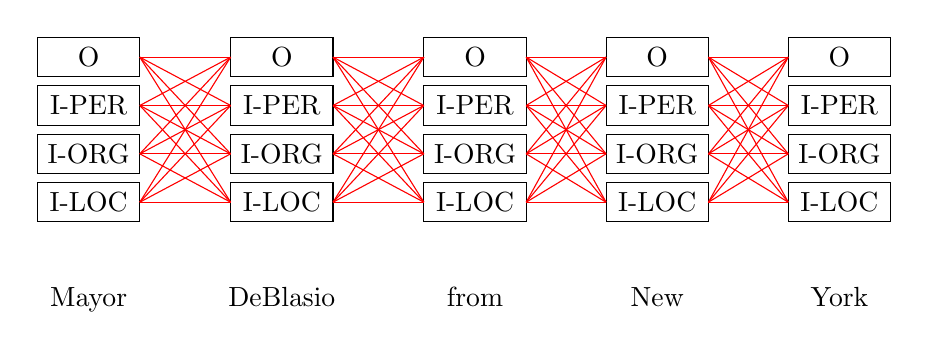
\begin{tikzpicture}
    \Lattice
    \foreach \i in {1,...,4} {
    \foreach \j in {1,...,4} {
    \draw[red] (network-\i-1.east) -- (network-\j-2.west);
    \draw[red] (network-\i-2.east) -- (network-\j-3.west);
    \draw[red] (network-\i-3.east) -- (network-\j-4.west);
    \draw[red] (network-\i-4.east) -- (network-\j-5.west);
    } }

    % \draw[red] (network-1-3.west) -- (network-1-2.east);
    % \draw[red] (network-1-3.west) -- (network-2-2.east); 
    % \draw[red] (network-1-3.west) -- (network-3-2.east);
    % \draw[red] (network-1-3.west) -- (network-4-2.east);

  \end{tikzpicture}
  \end{center}  
  
\end{frame}

\begin{frame}
  \begin{center}
   
  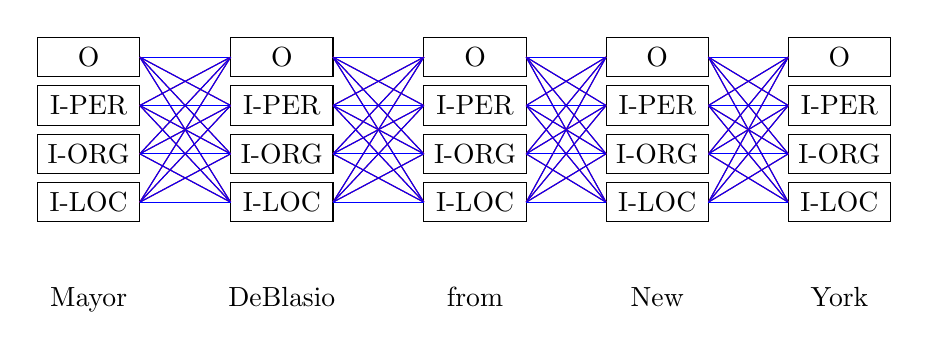
\begin{tikzpicture}
    \Lattice
    \foreach \i in {1,...,4} {
    \foreach \j in {1,...,4} {
    \draw<1->[red] (network-\i-1.east) -- (network-\j-2.west);
    \draw<2->[red] (network-\i-2.east) -- (network-\j-3.west);
    \draw<3->[red] (network-\i-3.east) -- (network-\j-4.west);
    \draw<4->[red] (network-\i-4.east) -- (network-\j-5.west);
    \draw<8->[blue] (network-\i-1.east) -- (network-\j-2.west);
    \draw<7->[blue] (network-\i-2.east) -- (network-\j-3.west);
    \draw<6->[blue] (network-\i-3.east) -- (network-\j-4.west);
    \draw<5->[blue] (network-\i-4.east) -- (network-\j-5.west);

    } }
  \end{tikzpicture}
  \end{center}  
\end{frame}


\begin{frame}
  \begin{center}
   
  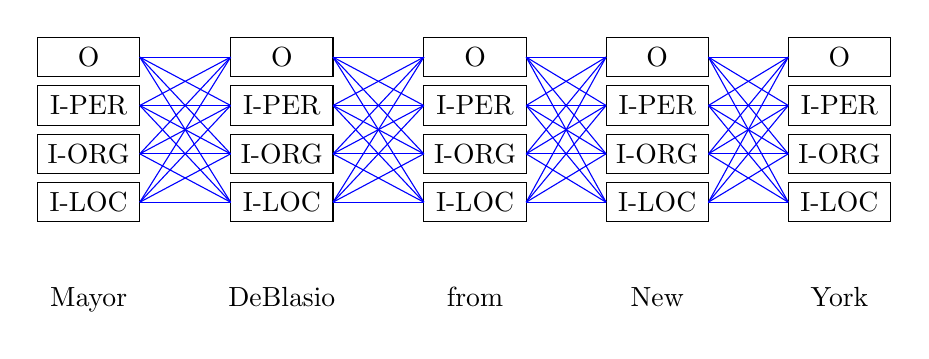
\begin{tikzpicture}
    \Lattice
    \foreach \i in {1,...,4} {
    \foreach \j in {1,...,4} {
    \draw<8->[blue] (network-\i-1.east) -- (network-\j-2.west);
    \draw<7->[blue] (network-\i-2.east) -- (network-\j-3.west);
    \draw<6->[blue] (network-\i-3.east) -- (network-\j-4.west);
    \draw<5->[blue] (network-\i-4.east) -- (network-\j-5.west);
    } }
  \end{tikzpicture}
  \end{center}  
  
\end{frame}


\begin{frame}{Forward Algorithm}
  \begin{algorithmic}
    \Procedure{Forward}{}
    \State{$\alpha \in \reals^{\{0,\ldots, n\} \times \mcC}$ initialized to $-\infty$ }
    \State{$\alpha[0, \langle s \rangle] = 0$}
    \For{$i = 1$ to $n$ }
    \For{$c_{i} \in \mcC$}
    \State{$\alpha[i, c_i] = \sum_{c_{i-1}} 
     \alpha[i-1, c_{i-1}] * \hat{\boldy}(c_{i-1})_{c_i}        
       $}
    \EndFor{}
    \EndFor{}
    \State{\Return{$\sum_{c_n\in\mcC} \alpha[n, c_n]$}}
    \EndProcedure{}
  \end{algorithmic}
\end{frame}


\begin{frame}{Backward Algorithm}
  \begin{algorithmic}
    \Procedure{Backward}{}
    \State{$\beta \in \reals^{\{1,\ldots, n+1\} \times \mcC}$ initialized to $-\infty$ }
    \State{$\beta[n+1, \langle s \rangle] = 0$}
    \For{$i = n$ to $1$ }
    \For{$c_{i} \in \mcC$}
    \State{$\beta[i, c_i] = \sum_{c_{i+1}} 
     \beta[i+1, c_{i+1}] * \hat{\boldy}(c_{i})_{c_i+1}        
       $}
    \EndFor{}
    \EndFor{}
    \State{\Return{$\sum_{c_1\in\mcC} \beta[1, c_1]$}}
    \EndProcedure{}
  \end{algorithmic}
\end{frame}





\begin{frame}{Marginals}

  \[M(c_i) =  \sum_{c_{1:n}} f(\boldx, c_{1:n}) \] 
  
  % \[ \frac{\partial M}{\partial } \]

\end{frame}


\begin{frame}{Probabilistic }
  \[ p(\boldy_i = c_i | \boldx) = \sum_{c_i} p( \boldy_i = \delta(c_i) | \boldx_{1:n})  \] 

  For the case of MEMM gives you just this. 


  For HMM
  \begin{eqnarray*}
     p(\boldy_i = c_i | \boldx) &=& \sum_{c_i} p( \boldy_i = \delta(c_i) | \boldx_{1:n})  \\
     &= & p(\boldy_i = c_i | \boldx) = \sum_{c_i} p( \boldy_i = \delta(c_i), \boldx_{1:n}) / p(\boldx_{1:n})   \] 
    
  \end{eqnarray*}


  How do you compute $p(\boldx_{1:n})$?
  % \[M(c_i) =  \sum_{c_{1:n}} f(\boldx, c_{1:n}) \] 
  
  % \[ \frac{\partial M}{\partial } \]

\end{frame}

\begin{frame}
  \[ p(\boldx_{1:n}) = \sum_{c_i}  \] 
\end{frame}


\begin{frame}{Edge Marginals}

  \[M(c_{i-1}, c_i) =  \sum_{c_{1:n}} f(\boldx, c_{1:n}) \] 
  
  % \[ \frac{\partial M}{\partial } \]

\end{frame}

\begin{frame}{}
  Is this the same forward-backward? 
\end{frame}


\begin{frame}{Viterbi}
  
  

\end{frame}



\section{Viterbi}


\end{document}
